	\documentclass[12pt]{article}
\usepackage{fullpage}
\usepackage{parskip}
\usepackage[round]{natbib}
\usepackage[utf8x]{inputenc} % keyboard input of accent marks
\usepackage[hyphens]{url} % formats URLs nicely
\usepackage{authblk}
\usepackage{booktabs} % for cleaner tables
\usepackage{graphicx}
\usepackage{comment}
\usepackage[capposition=top]{floatrow}
\usepackage[hidelinks]{hyperref} 				% to make nice links
\usepackage{xcolor}
\usepackage{enumitem}
\usepackage{amsmath}
\usepackage{amssymb}
\usepackage{wrapfig}
\usepackage{lscape}
\usepackage{threeparttablex}
\usepackage{chngcntr}

\hypersetup{
	colorlinks,
	linkcolor={red!50!black},
	citecolor={blue!50!black},
	urlcolor={blue!80!black}
}
\usepackage{setspace}
\usepackage{float}
\usepackage{array}
\newcolumntype{H}{>{\setbox0=\hbox\bgroup}c<{\egroup}@{}}

\usepackage{tabularx,ragged2e,booktabs}
%\newcolumntype{L}{>{\RaggedRight\arraybackslash}X} % ragge
\usepackage{grffile}
\usepackage{multirow}

\usepackage{array}
\newcolumntype{L}[1]{>{\raggedright\let\newline\\\arraybackslash\hspace{0pt}}m{#1}}
\newcolumntype{C}[1]{>{\centering\let\newline\\\arraybackslash\hspace{0pt}}m{#1}}
\newcolumntype{R}[1]{>{\raggedleft\let\newline\\\arraybackslash\hspace{0pt}}m{#1}}


\begin{document}
	
	
	\title{The Economic Payoff of
		Name Americanization: Replication Exercise}

	\author{Carlos Cardona Andrade\thanks{MRes at University of Warwick } } 


	\maketitle
	\begin{abstract}
		
		
Estimating the economic returns to cultural assimilation is pivotal in order to both understand migrants' behaviour in different countries and prepare effective policies for integrating them into the new socioeconomic background. This paper estimates the payoff of a key assimilation strategy during the age of Mass Migration: name Americanization. Findings suggest that the returns are nonnegligible and that they are driven by the migrants who face stronger barriers for occupation mobility.
		

		
	\end{abstract}
	


\onehalfspacing


\section{The Paper}

Migrants usually face a trade-off between assimilation and keeping their original identity. Thus, quantifying the economic returns to the process of assimilation is key for understanding both such tension and the population who self-selected themselves to assimilate into the new place. However, precisely because of the self-selection problem, estimating the returns are challenging. Using a digitized dataset of migrants in United States,  \cite{biavaschi2017economic} estimate the return of adopting a more American first name discarding the endogeneity concerns given the longitudinal nature of the data.  

\medskip

The data consist in a random sample of male immigrants who complete their naturalization procedure by 1930 in New York. They will exploit the fact that the process rest in two steps: the declaration of the intention to become an American citizen and a later petition for the naturalization. For both steps, they have the name of the male migrant at that stage and at the moment of his arrival, his occupation and aditional characteristics which will be discussed in the replication section. Table \ref{tab:table1} in the appendix section shows the share of migrants who changed their name by country. Among the final sample of 4083 immigrants, 31\% change their names in any of the stages. Due to the lack of wages information before 1940 census, the paper relies on the occupational score which is a measure of the median total income in 1950 dollars available in the IPUMS Census data \citep{ruggles2015integrated}.

\medskip

The authors use several specifications in order to robustly estimate the returns. First of all, they control for characteristics which vary over time. Secondly, by estimating a first difference specification they cancel out time invariant characteristics which potentially could explain earnings increases. Thirdly, they focus on just migrants who changed their name ruling out unobserved differences with other sort of migrants. Finally, they compare migrants with the same name at birth for understanding name assimilation trend. Across all these estimation procedures, the paper  find positive and statistical significant returns lying between 3\% and 5\%. 

\medskip

As mentioned above, understanding which population adopt such assimilation strategies is also relevant. In order to do this, \cite{biavaschi2017economic} explore heterogeneous effects by type of migrant and height concluding that their findings are mainly driven by migrants who faced the harshest restrictions for labour mobility. Lastly, they performed several robustness checks such as lagging the name popularity, instrumenting name popularity with the Scrabble points of the name, redefining the outcome variable and discarding potentially discrepancies due to phonetic differences. 


\section{Literature Review}

The paper contributes to the literature of economic outcomes during the age of Mass Migration and cultural assimilation. Among the papers related to this topic, \cite{abramitzky2014nation} contributes immensely by linking several census across times in order to analyze the economic variables of migrants in a longitudinal setting. They prove that the prior thought about difficult conditions for the migrants were wrong finding that immigrants faced the same labour mobility patterns than Americans. The findings presenting in the following sessions would suggest that there is an upward bias in estimations using a linkage method since they are not considering migrants who changed their name and also experience more difficult barriers in US labour market.

\medskip

In addition to the paper, there are two studies specifically related to changing your name. Firstly, \cite{goldin2004making} studies the reasons behind women keeping their last name after marriage in the US. Using data from the New York times marriage announcements, Massachusetts birth records and Harvard alumni books they find that keeping the last name during the 70's and 80's was more common among college graduates and women that already had a reputation. However, there was a reduction in the share of name keepers in the 90´s. On the other hand, \cite{arai2009renouncing} do study the consequences of adopting a Swedish or neutral surname. They estimate a fixed effect model using all Asian, African and Slavic inmigrants during the 90's who change their name finding a sizeable and statistical significant effect. The effect is much stronger for women than for men possibly due to the perception that a woman with a Swedish surname has a higher social capital through marriage. 

\medskip

Altough the paper mentioned the linkage process in \cite{abramitzky2014nation}, the authors do not cite the more recent working paper \cite{abramitzky2016cultural} which updates and deepen the analysis related to the assimilation patterns of immigrants considering name Americanization through different generations. Using names from several census previous to 1930 and birth certificate records of California since 1980, they find that for new generations it takes in average 28 years for closing the gap between foreing names and native names. Considering the results of this paper, it means that the convergence rate of foreign names potentially is even faster since the migrants under the worst conditions are changing their name since the first generation. 

\section{Replication}

In this section, I replicate the main results, the heterogeneity analysis and the robustness checks which correspond to table 3, 4 and 5 respectively. Moreover, additional tables and figures are in the appendix section.

\medskip

 The main purpose of the paper is estimating the returns of Americanizing your name. Thus, they propose an Americanization index which measure the popurality of a particular name with respect to the most common American names. The construction of this metric follows the next equation:

$$A_{it}=\frac{W^k_{it}}{max(W^1,...,W^k)} \quad \text{where} \quad  W_{it}=\sum_j\mathbf{1}(Name_{it}=Name_j)$$

for all $k$ names among $j$ Americans. The values of the index $A_{it}$ are between 0 and 1, where 0 means that any American has that particular name and 1 is that the name is the most common across Americans in year $t$. In other words, the paper want to estimate if increases in $A_{it}$ lead to increases in occupational based earnings. Given that individuals could change their names at different stages, the sample is divided by people who change their name before declaration (Early Americanizers),  people who change their name after declaration (Late Americanizers), migrants who do not change their name (Keepers) and those who change their name for less American names (Others). Figure \ref{fig:fig2} shows the average of the logarithm of the occupational score divided by group and at different stages of the declaration process. 

\medskip

The paper estimates the effect of name Americanization through the following specification equation for different models:

\begin{equation}
y_{it}=\beta_0+\beta_1A_{it}+\mathbf{x'}_{it}\gamma+c_i+\varepsilon_{it}
\end{equation}

where $y_{it}$ is the logarithm of the occupational score for individual $i$ in year $t$ and $A_{it}$ is our main explanatory variable. The vector $\mathbf{x_{it}}$ includes characteristics such as marital status, a dummy if $i$ has an American partner and also if he has an American child, the number of children, a dummy if he resides outside NY, years since migration, a dummy if he arrived previous to 1921, country of birth and district of residence. The last three variables are also interacted with years since migration in order to consider specific assimilation patterns related to those variables. There is also a time invariant component $c_i$ for each individual $i$ and $\varepsilon_{it}$ is the error term.

\medskip 

\subsection{Main Results}
Table \ref{tab:table3} shows results of the estimation equation (1) under different models. Column 1 shows an OLS estimation finding that increasing your Americanization Name index is related to a significant return of 3.5\%. Being married and having either an American partner or child are also associated with positive returns while having children and living outside NY city are related to negative returns. Column 2 perform the estimation taking into account country and district of residence trends. The statistical significance of our coefficient of interest decrease but numerically is close to the previous result. Except for living outside NY, the sign and significance of the other covariates remain the same under this specification. Even though the authors report in the table that they control for the interaction between arriival prior 1921 and years since migration, in the original code such interaction is not included in the regression. However, the results remain the same. 

\medskip

Columns 3 and 4 take advantage of the longitudinal nature of the data by estimating equation (1) under a first difference setting. Increasing the popularity of your name is associated with a higher and more statistical significant return of 9.8\% in column 3 while other covariates lose their statistical significance except for having an American partner or children. The coefficient is double than in the OLS model and it increases even more after controlling for national and district trends. The next step is estimating the equation in first difference just for those individuals who changed their name discarding the self selection into name Americanization. The estimates shows a return close to 24\% after controlling for specific national trends. At the bottom of table \ref{tab:table3}, the predicted average return for the whole sample is 4.6\% for the whole sample and 10.3\% for name changers only. Finally, 

\subsection{Heterogeneity Analysis}

Overall, the main results find that OLS estimations are underestimating the economic payoff for name Americanization. In order to clarify if the results are driven by migrants who face more difficult restriction in US labour market, the authors estimate equation (1) by different groups. Due to the lack of socioeconomic background variables, the paper employes proxies to these variables such as country of origin and height. Migrants are divided by two categories: old and new migrants. The first group consist of German, Scandinavian, Irish and British migrants since this group arrived in the middle of the XIX century while migrants from Italy, Eastern European countries and Russiand arrived at the end of the century and they were also low-skilled workers. The authors also propose another proxy for social background: their height. It is well recognized that height is strongly correlated with wealth, therefore, the paper divides the sample between migrants that are higher (tall) and below (short) than the average American.


\input{"table3.tex"}




Table \ref{tab:table4} presents the results by groups across the different models. By dividing the sample between old and new migrants, it is clear that the payoff for name Americanization are much higher for new migrants while they are non significant for the old ones. The figures are 12.2\% for the FD estimator and 27.3\% among just name changers. Additionally, the returns are also non significant for tall immigrants. On the other hand, the results are between 5\% and 20\% for migrants shorter than the average American. This evidence corroborates that those migrants who faces more constraints are driving the overall results. Finally, the variable arrival prior to 1921 is defined as a dummy in the paper, nonetheless it is a continuous variable in the original data set. I run all the specifications after redefining this variable in order to convert it into a dummy. Some results slightly change in the second decimal but remain the same statistical significance. 

\input{"table4.tex"}


\subsection{Robustness Checks}

The authors carry on several robustness checks for which I replicate a few of them in table  \ref{tab:table5}. First of all, instead of using the name at birth, they use the name at the declaration of the intention for naturalization. In these specifications the paper do not exploit all the changes of name since people could change between the arrival and declaration. Despite the latter, the results are consistent with the baseline results for equation (1). For this table, my results for the first difference estimator does not concide with the presented in the paper. Instead of using the Americanization index calculated for the entire sample, they use the index estimated for name changers only. However the estimate is even more statistical significant but smaller.

\medskip

 The next robusness check consist in using a subsample just considering people who made the declaration within a time window less than 3 years after their arrival. This group of early declarants are cleaner than the original sample in the sense that you are reducing the potential confounder factor of labour experience on changing your name. Even though the sample size decreases reducing the statistical power, the estimates are positive and statistical significant for both the FD and the Name changers models. 
 
 \medskip
 
 The authors check the sensitivity of the results to the definition of the outcome variable. Rather than rely on the change of earnings according to a occupation score, they modify the outcome variable into an upgrading of the occupation. In that sense, the outcome measures the change of occupation from a low-skilled job into a high-skilled one. The results in columns 1-3 for this definition change are robust and show that changing the name improves the occupational mobility. 
 
 \medskip 
 
 Due to misspellings, the Americanization index could be potentially different among names that sound the same but are written in different ways. In order to avoid that and by using New York
 State Identification and Intelligence System Phonetic Code (NYSIIS) method, the Americanization index is going to change if the individual change his name into a phonetically different name. The results are consistent despite of the definition change of our main explanatory variable. The estimate for the name changers model is the greatest among all our specifications reaching a return of 34\%. 
 
 \input{"table5.tex"}
 
 \section{Extension}
 
 Several empirical papers have shown that exogeneous shocks could lead to an increase of the assimilation of a particular group of migrants. For instance, \cite{fouka2016backlash} evaluate the long-term impact of banning German language in US schools after the First World War. The author finds that there is a backlash as a response to this policy because in states applying the law, German names are more common among German migrants, intermarriage rates and German enlistment are lower. Moreover, after Pearl Harbor, Japanese migrants started naming their Children with more American names in order to offset the sentiment against this particular group of immigrants \citep{saavedra2018kenji}. It means that the context has a considerable relevance for the process of assimilation and, considering that US context was different before and after 1921 due to the immigration quotas \citep{ward2017birds}, exploring heterogeneous effects could shed light on differences between different type of migrants. 
 
 
 \medskip
 
 Table \ref{tab:ext} presents the results for this heterogeneous analysis for the OLS, the difference and the name changers only. By interacting the Americanization index with the dummy, the statistical significance of almost all the coeficients dissapear except for the estimation with just name changers controlling for country of birth and labour market specific trends. 
 
 




\input{"extension.tex"}



\bibliographystyle{apsr}
\bibliography{repbib}

\appendix
\counterwithin{table}{section}

\section{Appendix}


	\input{"table1.tex"}
		\input{"table2.tex"}
\begin{center}
	\begin{figure}[H]\caption{}\label{fig:fig1}
		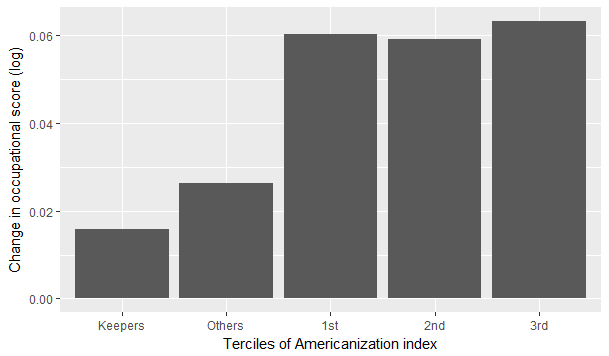
\includegraphics[width=150mm]{figure1.png}
	\end{figure}
\end{center}

\begin{center}
	\begin{figure}[H]\caption{}\label{fig:fig2}
		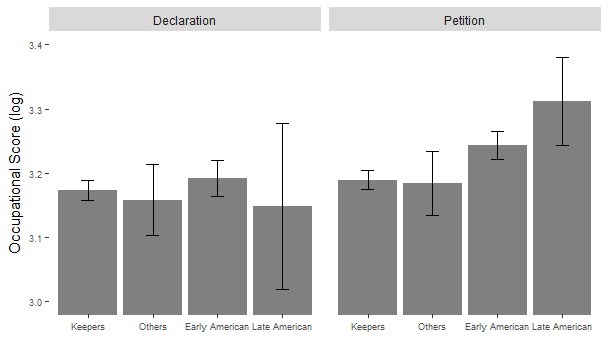
\includegraphics[width=150mm]{figure2.png}
	\end{figure}
\end{center}

\end{document}